\documentclass[a4paper,10pt]{article}
% Paquete para inclusión de gráficos.
\usepackage{graphicx}
% Paquete para definir el idioma usado.
\usepackage[spanish]{babel}
% Paquete para definir la codificación del conjunto de caracteres usado
% (latin1 es ISO 8859-1).
\usepackage[latin1]{inputenc}
\usepackage{hyperref}
% Include the listings-package
\usepackage{listings}  
\usepackage{pdfpages}


% Título principal del documento.
\title{	\ Trabajo Práctico Nº 0: Infraestructura Básica}
% Información sobre los autores.
\author{	Sebastian Ripari, \textit{Padrón Nro. 96453}\\
            \texttt{sebastiandanielripari@hotmail.com }\\\\
            Cesar Emanuel Lencina, \textit{Padrón Nro. 96078}\\
            \texttt{cel_1990@live.com}\\\\
			Pablo Sivori, \textit{Padrón Nro. 84026}\\
            \texttt{sivori.daniel@gmail.com}\\\\               
            \texttt{\footnotesize 1º Entrega: 07/09/2017}\\
            \\\\\\\\\\\\\\\\\\
            \normalsize{2do. Cuatrimestre de 2017}\\ 
            \normalsize{66.20 Organización de Computadoras} \\
            \normalsize{Facultad de Ingeniería, Universidad de Buenos Aires} \\}
       
\date{}

\begin{document}
% Inserta el título.
\maketitle
% quita el número en la primer página
\thispagestyle{empty}
% Resumen
\begin{abstract}
En el presente trabajo práctico se describirán todos los pasos y 
conclusiones relacionadas al desarrollo e implementación de una versión en lenguaje C,
de la Criba de Eratóstenes. Y su posterior compilacion y ejecucion bajo el procesador MIPS.
\end{abstract}
\newpage{}
\tableofcontents
\newpage{}

\begin{flushleft}

\par\end{flushleft}
\section{{\normalsize Introducción}}

El objetivo del presente trabajo práctico es familiarizarse con el emulador gxemul mediante la implementacion de un programa que nos devuelva por stdout o en un archivo de salida, los números primos menores a un número natural N el cuál es ingresado por parámetro.

\section{{\normalsize Entorno de trabajo}}
Mediante el emulador Gxemule pudimos simular una DEC Station 5000/200 con un microprocesador MIPS de 32 Bits, corriendo un sistema 
operativo NetBSD/pmax.

\subsection{{\normalsize Lenguaje}}

Como lenguaje de implementación se eligio C ya que el mismo permite una alta portabilidad entre 
diferentes plataformas. El desarrollo del programa se realizó usando editores de texto 
(gedit,vim, kwrite y sublime) y compilando los archivos fuente con 
\htmladdnormallink{GCC}{http://gcc.gnu.org/} que viene en linux. Ya que esta compilador es compatible
con el sistema operativo NetBSD y con la arquitecura MIPS.
Para compilar, ejecutar el siguiente comando:

\begin{tabbing}
------- \= ----- \= \kill
\> \textbf{\emph{\$ make}}\\ 
\end{tabbing}

\subsection {{\normalsize Descripción del programa}}

Por empezar tenemos un archivo llamado \texttt{erat.c} que contiene la funcion
\texttt{main}, aqui lo primero que hacemos es la validacion de los argumentos, mediante 
una funcion llamada \texttt{validarArgumentos}. Caso de ingresarse algo invalido 
el programa no continuara, y retornara un valor distinto de 0, osea un codigo de error. Caso contrario, 
se llama a la funcion \texttt{realizarAccion} y aqui comienza el procesamiento de calcular 
la cantidad de numeros primos, entre 2 y el numero \texttt{tope} ingresado. Basicamente lo que hacemos es 
crear un array que contiene todos los numeros entre 2 y el numero ingresado, el \texttt{tope}. 
y luego le aplicamos a este array el algoritmo de la Criba de Erastostenes, mediante la funcion \texttt{encontrarNumerosPrimos},
que en las posiciones del array donde no hay un numero primo setea un cero.
Para luego tomar este array desde una funcion que se llama \texttt{imprimirPorPantalla}, y aqui imprimir todos los numeros distintos
de cero, que son los primos.

\subsubsection {{\normalsize Errores posibles}}

\begin{enumerate}
\item Comando invalido: Cuando se invoca al programa con flags inexistentes o escritos de forma desordenada. El programa retorna 2.
\item Fuera de rango: Cuando se ingresa un numero menor o igual que 1. El programa retorna 1. 
\end{enumerate}

\subsubsection {{\normalsize Corridas de prueba}}

\begin{enumerate}
\item Caso N = -5
El programa no imprime nada y retorna el codigo de error 1.
\item Caso N = 1
El programa no imprime nada y retorna el codigo de error 1. 
\item Caso N = 10
El programa imprime: 2 3 5 7 y retorna el codigo de exito 0.
\item Caso N = 50
El programa imprime 2 3 5 7 11 13 17 19 23 29 31 37 41 43 47 y retorna el codigo de exito 0.
\item Caso N = 100
El programa imprime 2 3 5 7 11 13 17 19 23 29 31 37 41 43 47 53 59 61 67 71 73 79 83 89 97 y retorna el codigo de exito 0.  
\end{enumerate}
	
\newpage
\section{{\normalsize El código fuente, en lenguaje C:}}

	\lstinputlisting[language=C, basicstyle=\tiny]{../erat.c}
	\lstinputlisting[language=C, basicstyle=\tiny]{../erat.h}
	\lstinputlisting[language=C, basicstyle=\tiny]{../eratfunc.c}
	\lstinputlisting[language=C, basicstyle=\tiny]{../eratfunc.h}	

\newpage
\newpage
\newpage

\section{{\normalsize El código assembly generador por GCC en el simulador es:}}

	\lstinputlisting[language={[x86masm]Assembler}, firstline=1, lastline=45, basicstyle=\small]{../erat.s}
 	\lstinputlisting[language={[x86masm]Assembler}, firstline=1, lastline=45, basicstyle=\small]{../eratfunc.s}
 
\newpage{}
\section{{\normalsize Conclusiones}}

\begin{enumerate}
\item Si bien lo solicitado por el programa no era excesivamente difícil,
la realización completa del TP llevó cierta dificultad al tener que
realizarlo en el contexto solicitado: alta portabilidad, desarrollo
en C, e informe hecho en LaTeX. 
\item En el primer caso la dificultad radicaba en tener configurado 
y funcionando el GXEmul dentro de un Linux, y lograr que en ambos casos 
el programa compile y corra sin problemas. 
\item Debido a nuestro desconocimiento con LaTeX, tuvimos que 
invertir tiempo en encontrar forma de realizar el presente documento 
de la manera más correcta posible 
\item En cuanto al trabajo grupal en si mismo, no hubo inconvenientes de
ningún tipo ya que al ser el grupo relativamente chico y tener conocimiento
del manejo del versionado de un proyecto ante cambios ingresado por
los integrantes (por medio del GIT), la introducción de modificaciones
y correcciones fué fluida. 
\end{enumerate}

\newpage
\section{{\normalsize Enunciado del trabajo practico}}

	%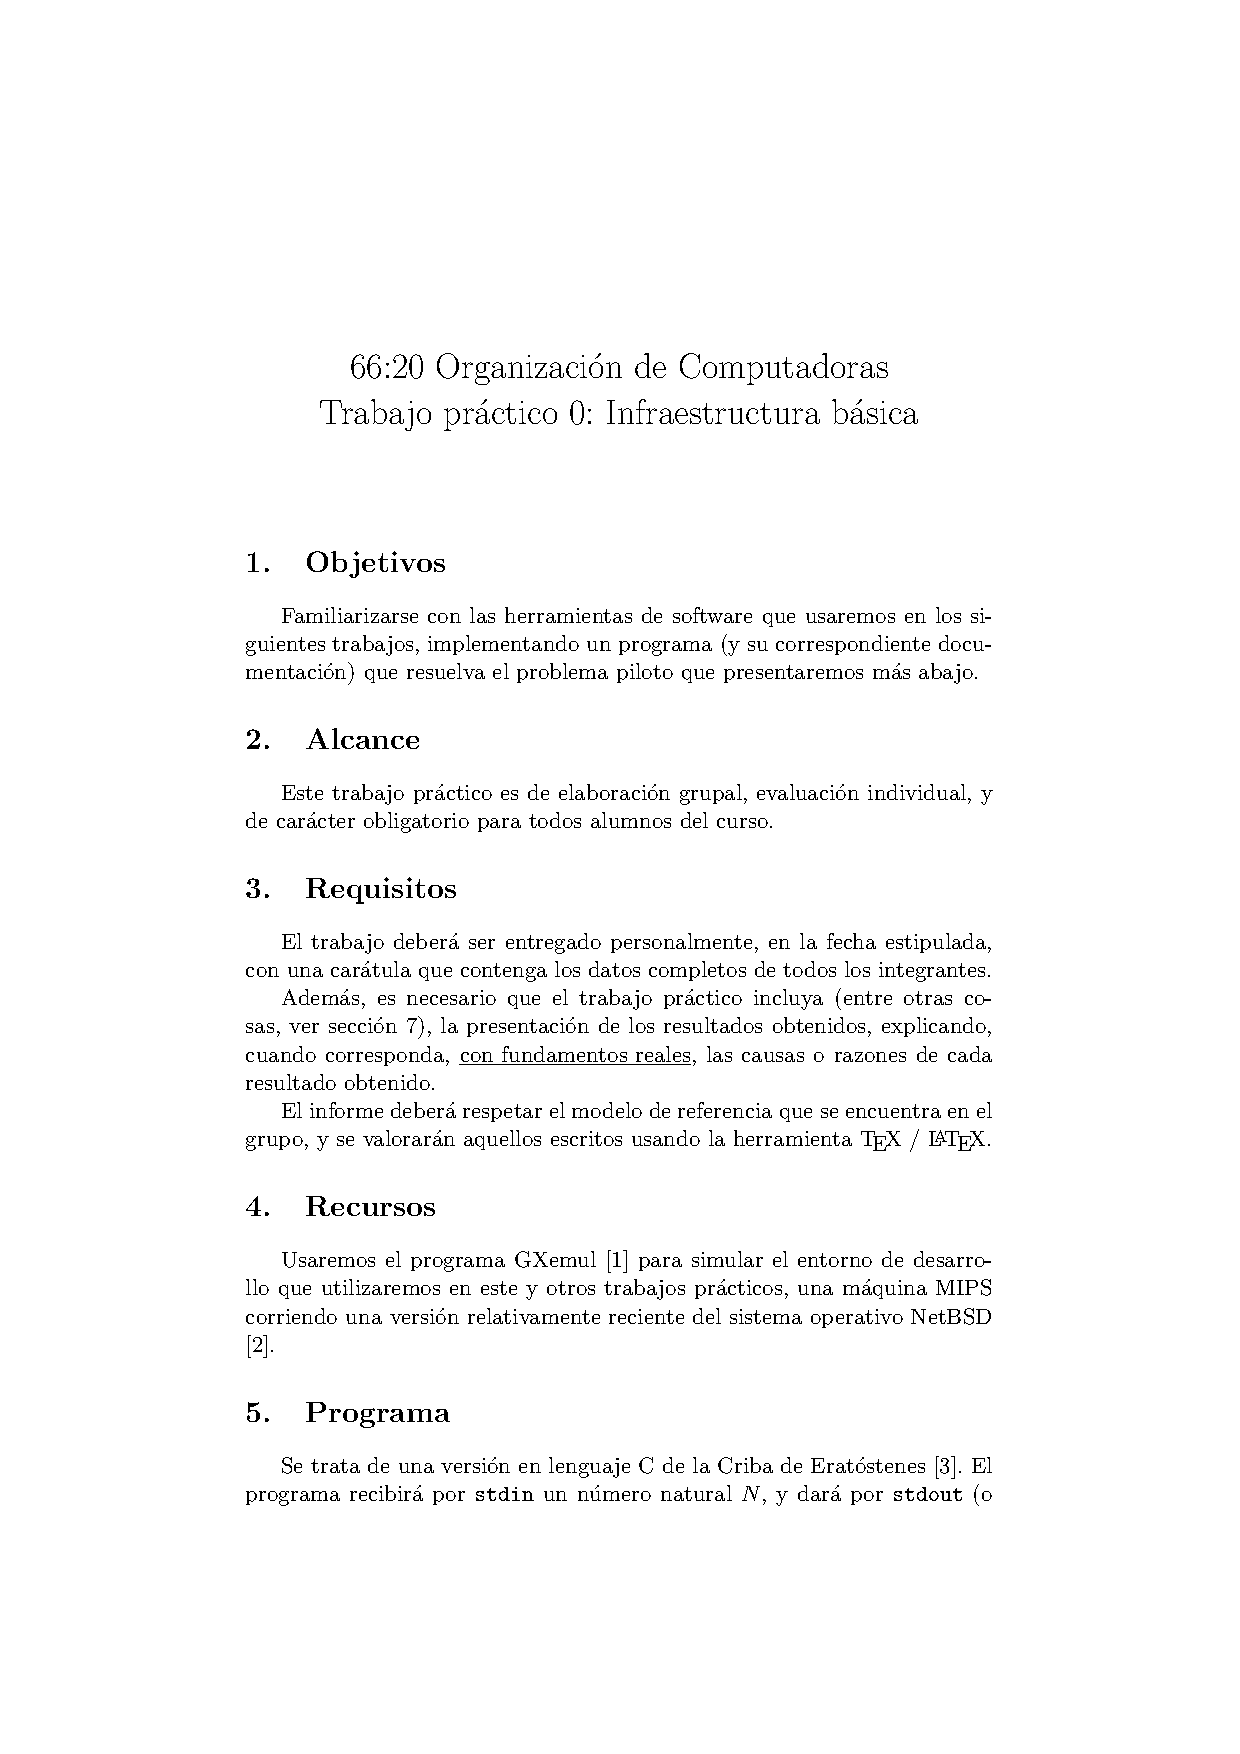
\includegraphics[width=0.8\textwidth]{enunciado.pdf}
	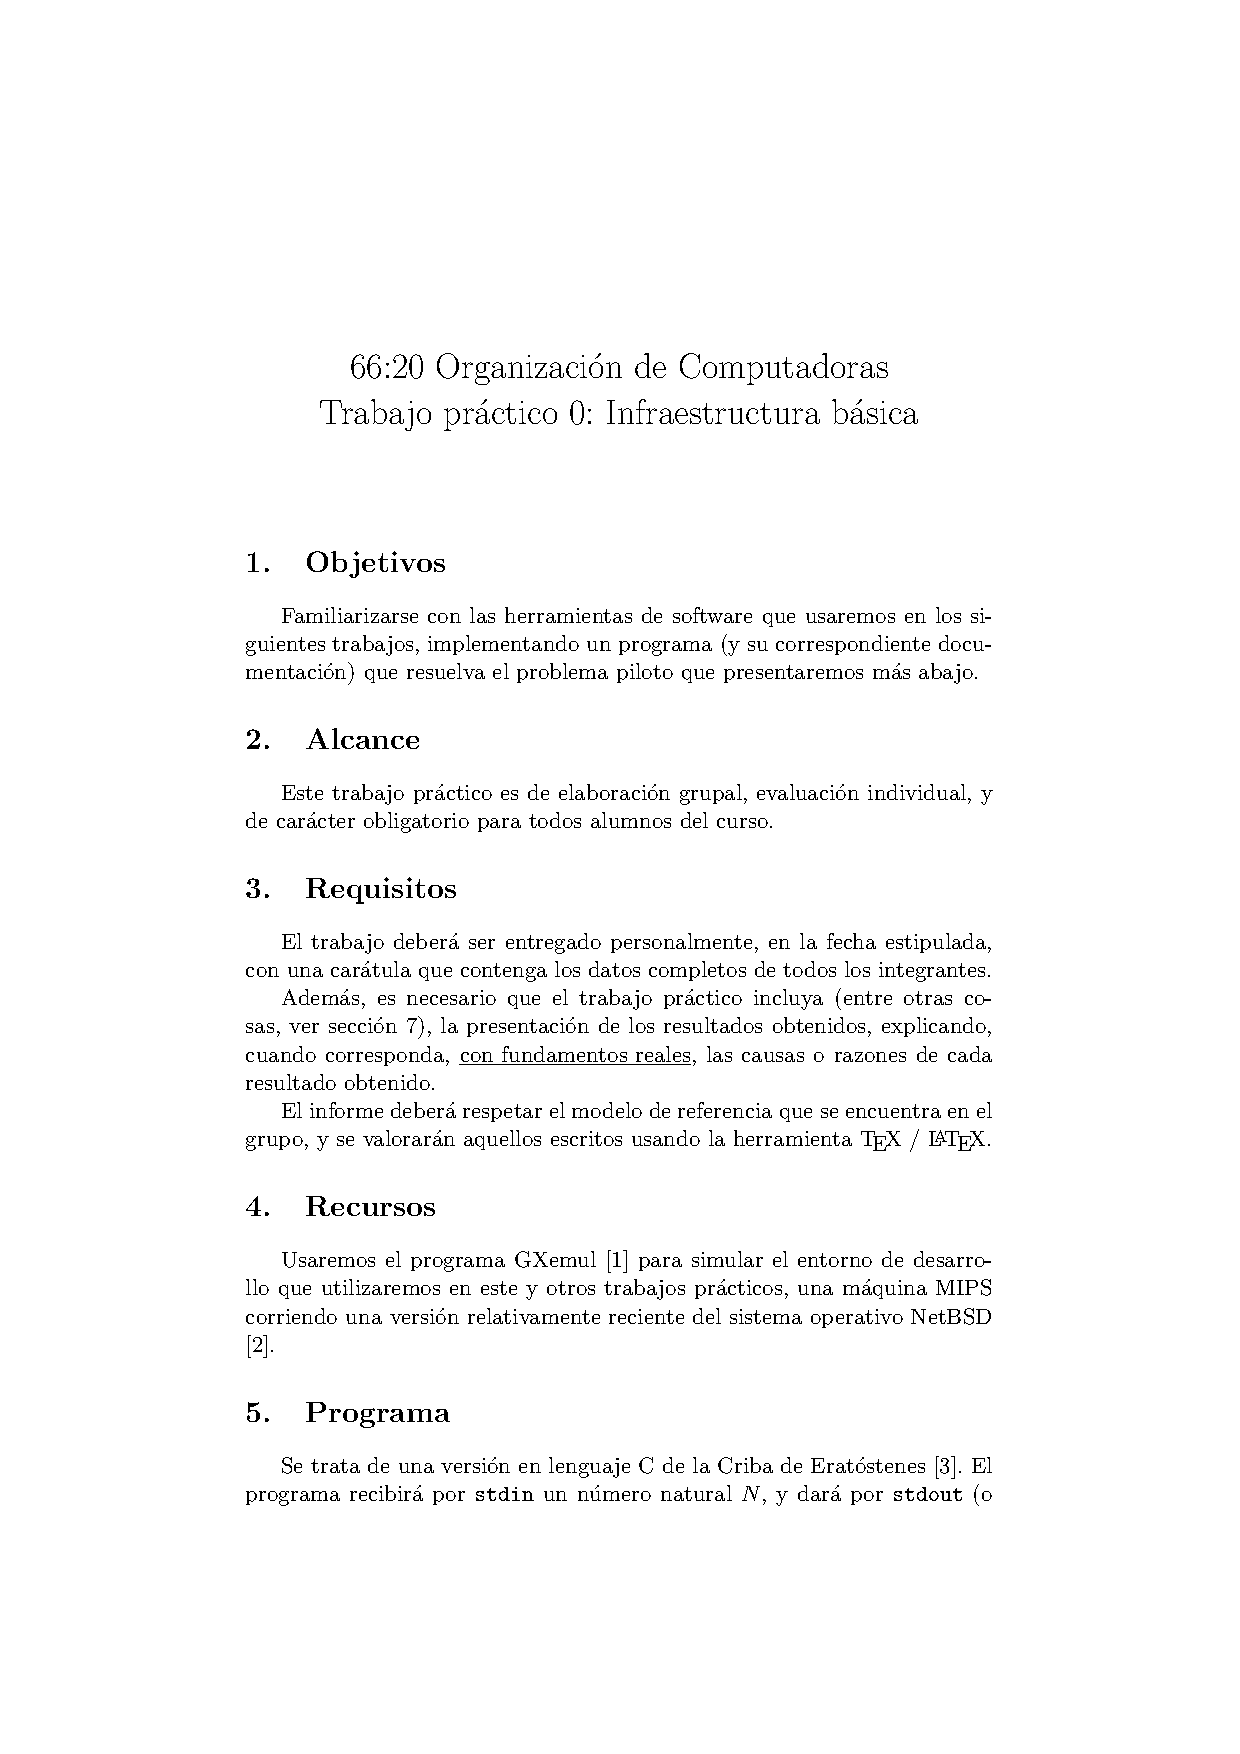
\includepdf[pages={1-},scale=0.75]{enunciado.pdf}


\bibliographystyle{plain}
\nocite{*}
\end{document}
